\documentclass[aspectratio=169,11pt]{beamer}
\input{../../../../theme/ksa-theme.tex}
\setbeamerfont{title}{series=\bfseries,size=\fontsize{24}{30}\selectfont}
\setbeamerfont{subtitle}{series=\bfseries,size=\fontsize{14}{18}\selectfont}
\setbeamerfont{author}{size=\normalsize}
\setbeamerfont{institute}{size=\small}
\graphicspath{{figs/}{../../../../assets/}}
\makeatletter
\newcommand{\markpage}[1]{\protected@write\@auxout{}{\string\newlabel{#1}{{\the\c@framenumber}{}}}\hypertarget{#1}{}}
\newcommand{\pref}[1]{\hyperlink{#1}{\textcolor{ksagolddk}{(p.\ref{#1})}}}
\makeatother

\renewcommand{\ksacredit}{Machine Learning 1 \,\textperiodcentered\, 정규화와 표준화}
\title{정규화와 표준화}
\subtitle{Min-Max Normalization · Z-score Standardization --- 데이터를 직접 열어 보기}
\author{Machine Learning 1}
\institute{한국과학영재학교 (KSA)}
\date{}
\begin{document}
\begin{frame}[plain,noframenumbering]\titlepage\end{frame}

% --- 오늘의 질문
\begin{frame}{오늘의 질문}
\vfill
\centering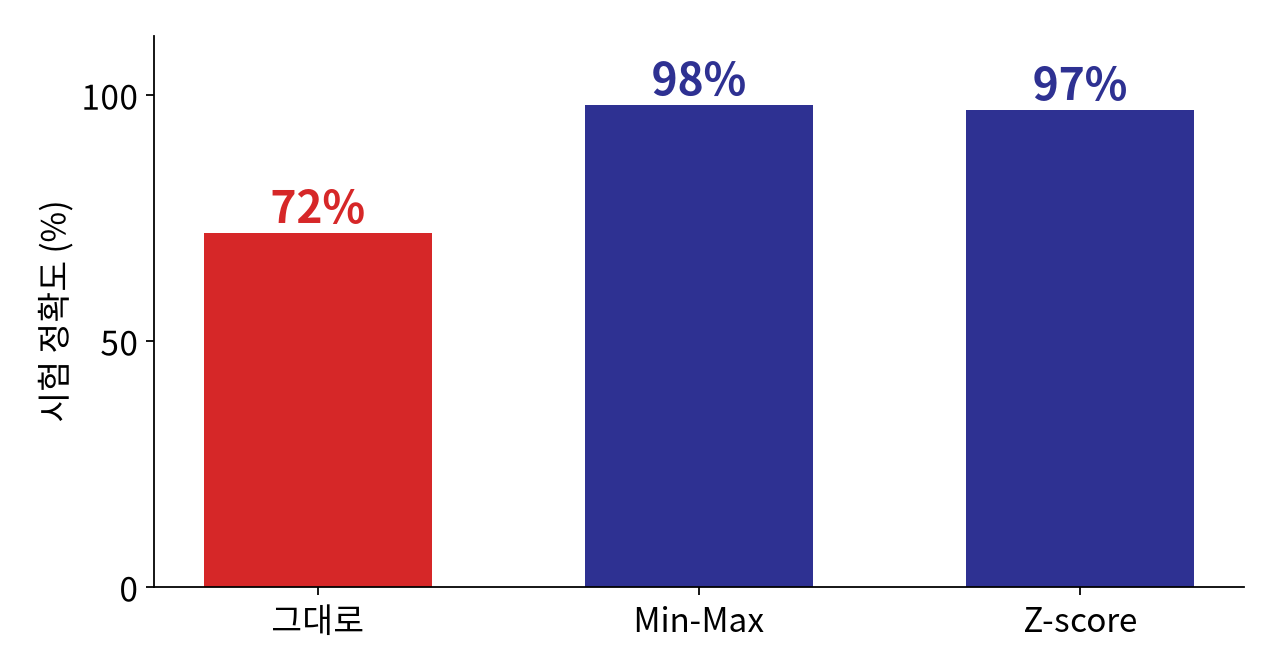
\includegraphics[width=0.6\linewidth]{fs_hook.png}\par\vskip0.3em
{\large 같은 신경망, 같은 와인 데이터. \kq{성분 값을 그대로 넣으면 72\%}, 정규화하면 \kb{98\%}}
\vfill
\note{와인 178병의 성분을 보고 품종 세 가지를 맞히는 신경망입니다. 모델도 같고 학습 방법도 같습니다. 바뀐 건 하나, 입력 값을 그대로 넣었느냐, 정규화해서 넣었느냐입니다. 그대로 넣으면 시험 정확도가 72퍼센트, 정규화하면 98퍼센트입니다. 시드를 10번 바꿔 평균 낸 값입니다. 숫자 몇 개를 빼고 나눈 것뿐인데 왜 이렇게 차이가 날까요? 오늘은 그 이유를 보고, 이미지, 글, 시계열, 소리, 비디오 데이터에서는 각각 무엇을 맞춰야 하는지 직접 데이터를 열어 봅니다.}
\end{frame}

% --- 성분 범위
\begin{frame}{와인 한 병 = 성분 값 13가지, 범위가 제각각}
\vfill
\centering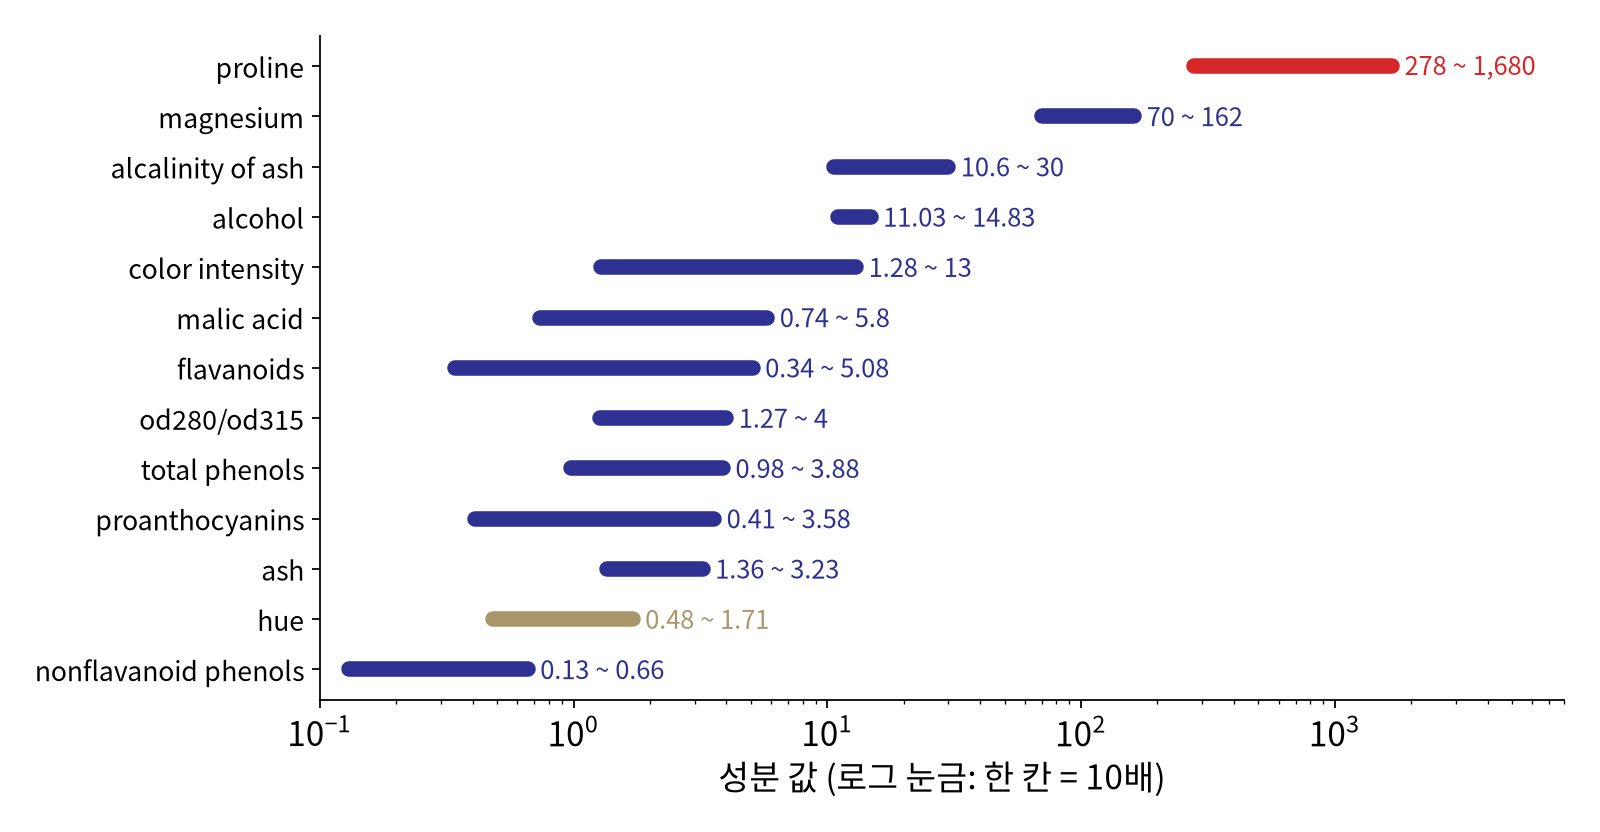
\includegraphics[width=0.78\linewidth]{fs_ranges.png}\par\vskip0.2em
{\large \kq{프롤린 278 $\sim$ 1,680}, \textcolor{ksagolddk}{\textbf{색조 0.48 $\sim$ 1.71}}: 천 배 넘게 차이 난다}
\vfill
\note{와인 한 병마다 알코올, 마그네슘, 프롤린, 색조 같은 성분 값이 13가지 있습니다. 가로축이 로그 눈금이라 한 칸이 10배입니다. 맨 위 빨간 막대 프롤린은 278에서 1,680, 아래쪽 색조는 0.48에서 1.71입니다. 단위가 다르니 크기도 제각각입니다. 사람은 단위를 보고 알아서 읽지만, 모델은 숫자만 봅니다.}
\end{frame}

% --- 뉴런
\begin{frame}{뉴런 하나가 하는 일}
\vfill
\centering
\begin{columns}[c]
\column{0.42\textwidth}\centering
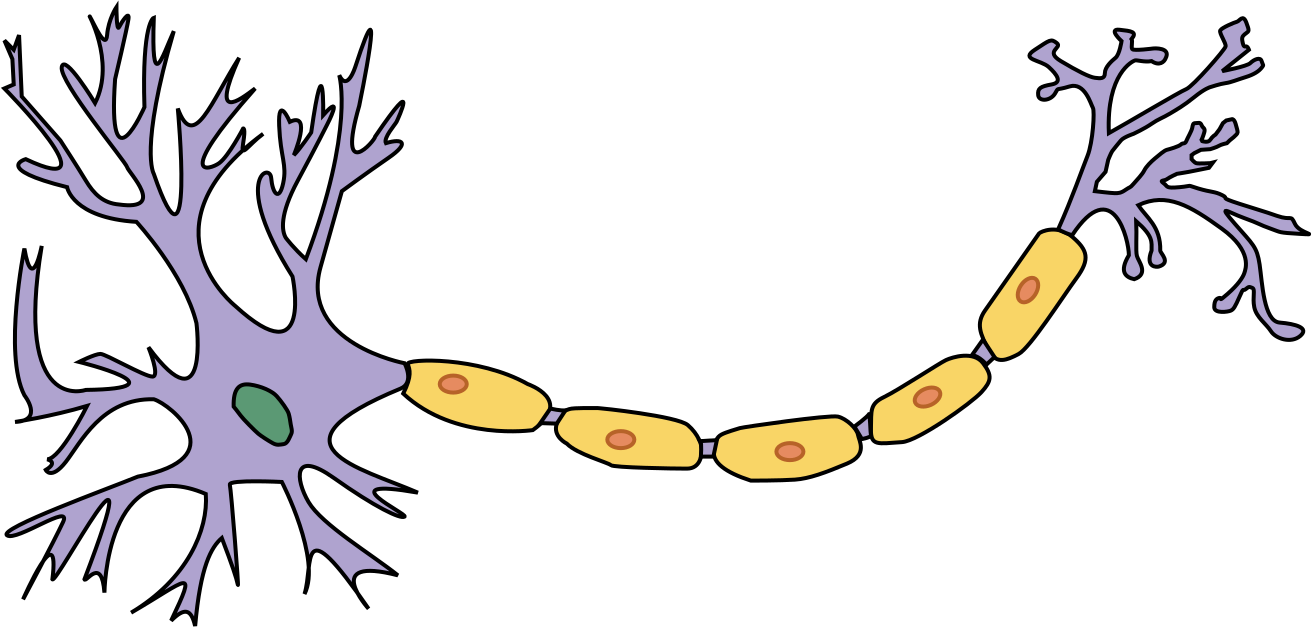
\includegraphics[width=\linewidth]{fs_neuron.png}
\column{0.54\textwidth}
{\LARGE\[ \text{output} = \tanh(\textcolor{ksablue}{w}\cdot x + b) \]}\vskip0.6em
{\large $x$ = 성분 값 13개 (데이터)\\[0.4em]
$\textcolor{ksablue}{w}$ = 뉴런이 \kb{학습할 가중치} 13개}\\[0.8em]
PyTorch \texttt{nn.Linear(13, 16)} 의 $w$ 는 처음에\\
\kb{$-0.28 \sim 0.28$} 사이 작은 난수 ($\pm 1/\sqrt{13}$)
\end{columns}
\vfill
\note{뉴런은 뇌세포처럼 입력 x에 가중치 w를 곱해 다 더하고, 탄젠트 에이치 같은 곡선을 거쳐 내보냅니다. 여기서 x는 데이터, 와인 성분 값이고, w는 뉴런이 학습할 변수입니다. 파이토치의 nn.Linear는 w를 마이너스 0.28에서 0.28 사이 작은 난수로 시작합니다. 입력이 13개라서 1 나누기 루트 13입니다. 즉 처음 w는 0 근처의 작은 수인데, x는 1,000이 넘을 수 있습니다.}
\end{frame}

% --- 계산
\begin{frame}{와인 1번 병을 그대로 넣으면}
\markpage{rawsum}
\vfill
\centering
{\large
\begin{tabular}{lrcrcr}
\textbf{성분} & \textbf{값 $x$} & & \textbf{가중치 $w$} & & \textbf{$x \times w$}\\\hline\\[-0.8em]
프롤린 & \kq{1,065} & $\times$ & 0.15 & $=$ & \kq{162.15}\\
마그네슘 & 127 & $\times$ & 0.05 & $=$ & 6.56\\
알코올 & 14.23 & $\times$ & 0.11 & $=$ & 1.57\\
색조 & 1.04 & $\times$ & $-0.16$ & $=$ & $-0.17$\\
나머지 9개 $+\,b$ & & & & & $-1.98$\\\hline\\[-0.8em]
\multicolumn{5}{l}{\textbf{합} $w\cdot x + b$} & \kq{168.13}
\end{tabular}}\vskip0.8em
{\Large $\tanh(168.13) = \kq{1.00}$}\quad 프롤린 하나가 합을 다 차지한다\\[0.3em]
{\scriptsize $w$ 는 반올림해 적었고, 곱은 반올림 전 값으로 계산 (seed 0, 4번 뉴런)}
\vfill
\note{와인 1번 병을 그대로 넣어 봅시다. 프롤린 1,065에 가중치 0.15를 곱하면 162입니다. 마그네슘은 6.6, 알코올은 1.6, 색조는 0.2도 안 됩니다. 나머지 아홉 개와 b를 다 더해도 마이너스 2 정도. 합은 168입니다. 탄젠트 에이치에 168을 넣으면 1.00, 곡선 끝에 붙어 버립니다. 사실상 프롤린 하나만 보고 있는 셈입니다.}
\end{frame}

% --- 포화
\begin{frame}{12병 모두 출력 1.00: 기울기 0, 배우지 못한다}
\vfill
\centering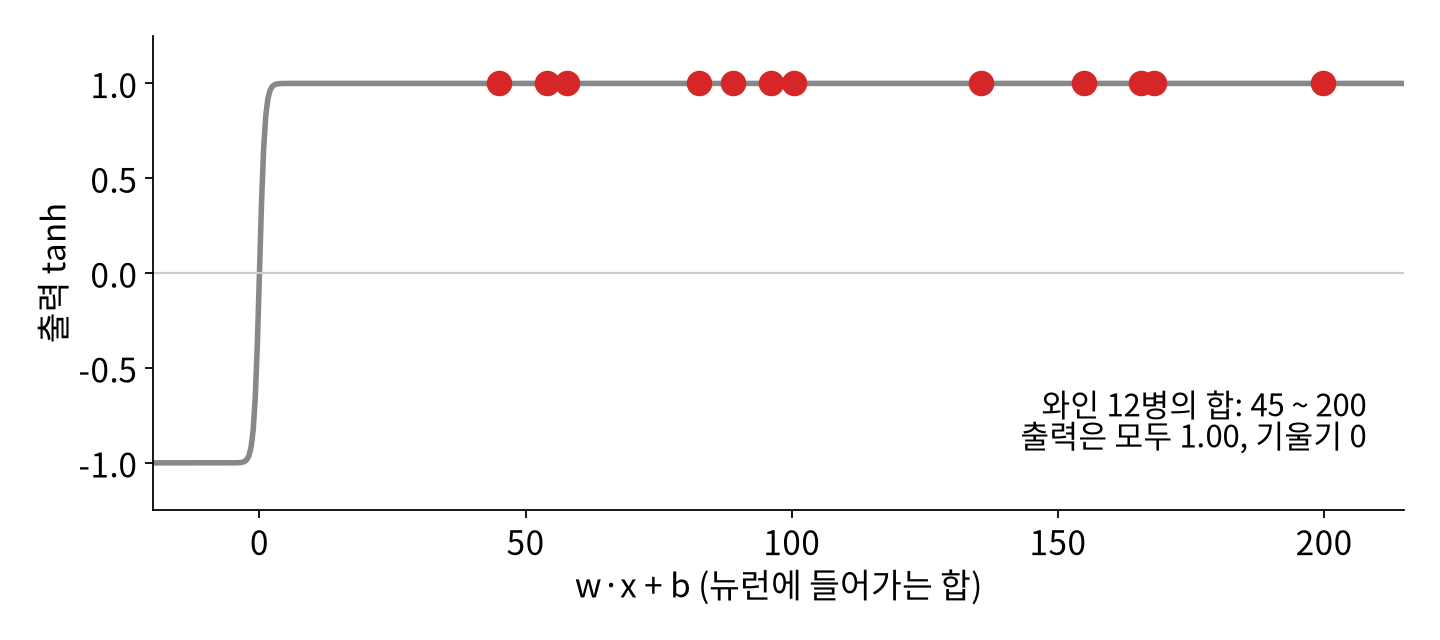
\includegraphics[width=0.74\linewidth]{fs_tanh_raw.png}\par\vskip0.3em
{\large 곡선이 평평한 곳 = \kq{기울기 0}. 학습 전 뉴런 출력의 \kq{98\%}가 이렇게 막혀 있다}
\vfill
\note{1번 병만 그런 게 아닙니다. 다른 와인 12병을 넣어 보면 합이 45에서 200 사이, 출력은 모두 1.00입니다. 곡선이 평평한 곳에 있으니 기울기가 0입니다. 기울기는 w를 어느 쪽으로 얼마나 고칠지 알려 주는 신호인데, 이게 0이면 학습이 안 됩니다. 학습 시작 때 은닉층 출력의 98퍼센트가 절댓값 0.99를 넘는, 이렇게 막힌 상태였습니다.}
\end{frame}

% --- 맞추면
\begin{frame}{성분마다 분포를 맞추면}
\vfill
\centering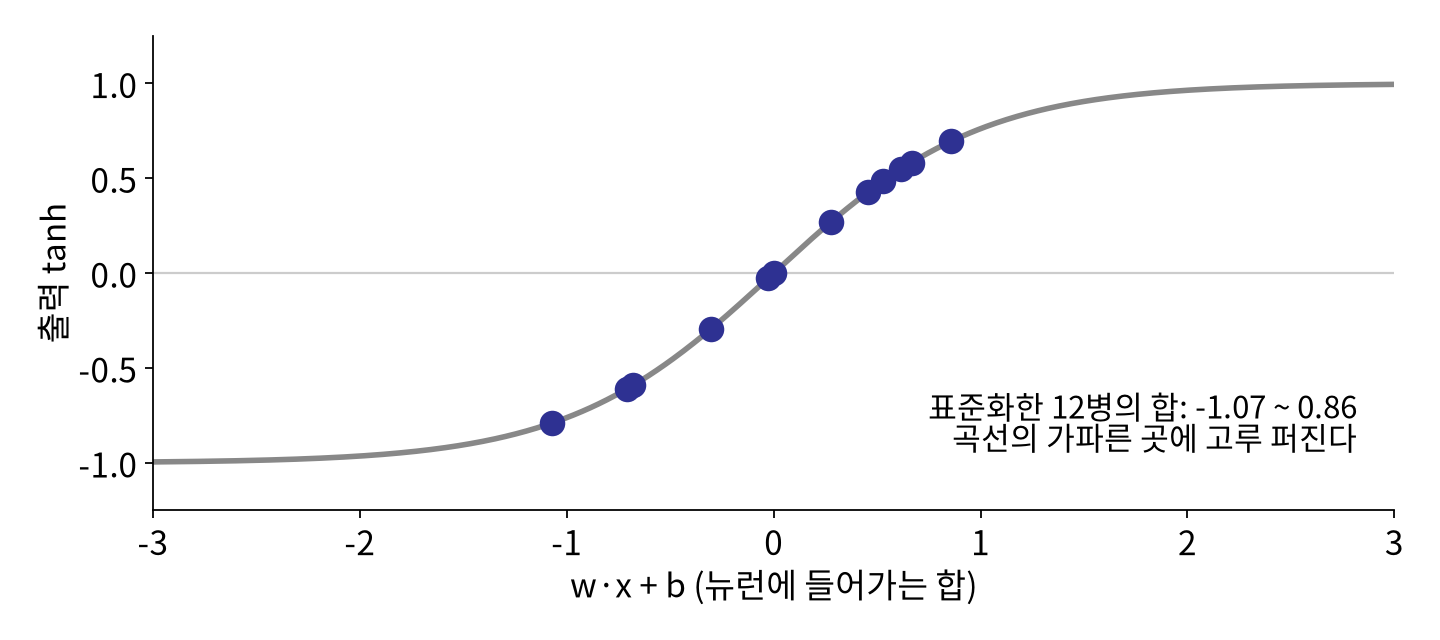
\includegraphics[width=0.74\linewidth]{fs_tanh_z.png}\par\vskip0.3em
{\large 프롤린 1,065 $\to$ \kb{1.01}. 합 \kb{0.67}, 출력 \kb{0.58}: 곡선의 가파른 곳에서 신호가 산다}
\vfill
\note{이번에는 성분마다 분포를 맞춰서 넣습니다. 방법은 곧 보겠습니다. 프롤린 1,065는 1.01이 되고, 다른 성분도 모두 0 근처의 비슷한 크기가 됩니다. 1번 병의 합은 0.67, 출력은 0.58입니다. 12병이 곡선의 가파른 곳에 고루 퍼집니다. 기울기가 살아 있으니 학습이 됩니다.}
\end{frame}

% --- Min-Max
\begin{frame}{방법 1. Min-Max 정규화: 0 $\sim$ 1 로}
\vfill
\centering
{\LARGE\[ x' = \frac{x - \textcolor{ksablue}{\min}}{\textcolor{ksablue}{\max} - \textcolor{ksablue}{\min}} \]}\vskip0.4em
{\large 성분마다 따로: 가장 작은 값 $\to$ 0, 가장 큰 값 $\to$ 1}\vskip1em
{\Large 프롤린 1,065: \quad $\dfrac{1065 - \textcolor{ksablue}{278}}{\textcolor{ksablue}{1680} - \textcolor{ksablue}{278}} = \dfrac{787}{1402} = \kb{0.56}$}\vskip1em
{\small 쓰기 좋은 곳: 이미지 픽셀처럼 \textbf{범위가 정해진 값} (0 $\sim$ 255 $\to$ 0 $\sim$ 1)}
\vfill
\note{첫 번째 방법은 Min-Max 정규화입니다. 성분마다 따로, 가장 작은 값을 빼고 범위로 나눕니다. 그러면 가장 작은 값은 0, 가장 큰 값은 1이 됩니다. 프롤린 1,065는 278을 빼서 787, 범위 1,402로 나누면 0.56입니다. 이미지 픽셀처럼 0에서 255로 범위가 정해진 값에 잘 맞습니다.}
\end{frame}

% --- Z-score
\begin{frame}{방법 2. Z-score 표준화: 평균 0, 표준편차 1 로}
\markpage{zscore}
\vfill
\centering
{\LARGE\[ z = \frac{x - \textcolor{ksablue}{\mu}}{\textcolor{ksared}{\sigma}} \]}\vskip0.2em
{\large $\textcolor{ksablue}{\mu}$ = 평균 (mean), \quad $\textcolor{ksared}{\sigma}$ = 표준편차 (standard deviation), \quad 성분마다 따로}\vskip1em
{\Large 프롤린 1,065: \quad $\dfrac{1065 - \textcolor{ksablue}{747}}{\textcolor{ksared}{314}} = \kb{1.01}$}\vskip0.6em
{\large ``평균보다 \textbf{표준편차 1개만큼} 많다''}\vskip0.8em
{\small 보통은 이것을 쓴다. 튀는 값 하나가 있어도 Min-Max 보다 덜 흔들린다}
\vfill
\note{두 번째는 Z-score 표준화입니다. 성분마다 평균을 빼고 표준편차로 나눕니다. 프롤린의 178병 평균은 747, 표준편차는 314입니다. 1,065에서 747을 빼면 318, 314로 나누면 1.01. 평균보다 표준편차 한 개만큼 많다는 뜻입니다. 결과는 평균 0, 표준편차 1이 됩니다. Min-Max는 가장 큰 값 하나가 튀면 나머지가 전부 0 근처로 눌리는데, Z-score는 덜 흔들립니다. 그래서 특별한 이유가 없으면 보통 Z-score를 씁니다. 참고로 여기 표준편차는 n으로 나눈 값, numpy의 std 기본값입니다.}
\end{frame}

% --- 모양은 그대로
\begin{frame}{모양은 그대로, 눈금만 바뀐다}
\vfill
\centering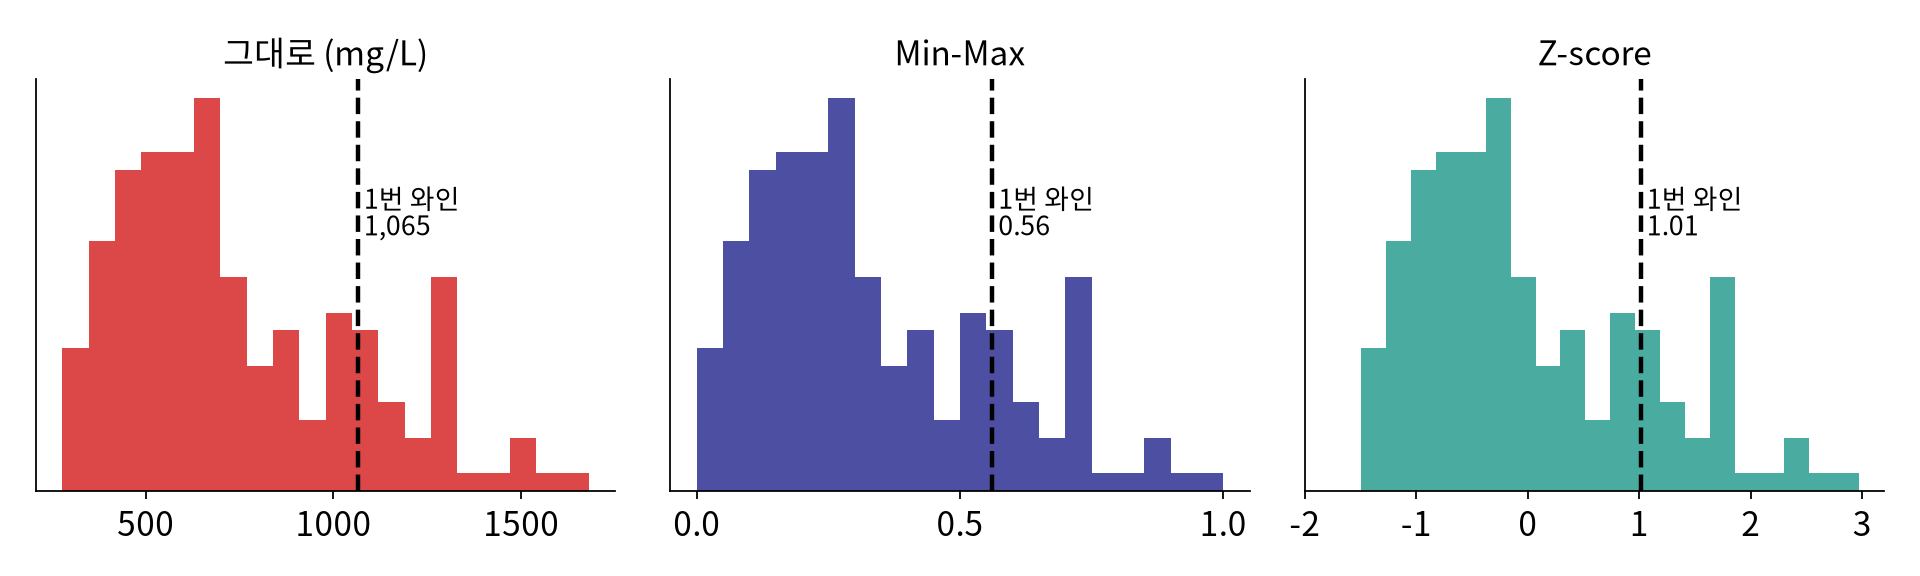
\includegraphics[width=0.92\linewidth]{fs_hist3.png}\par\vskip0.4em
{\large 프롤린 178병의 분포. 빼고 나누기만 해서 \kb{순서와 모양은 그대로}}\\[0.3em]
{\small 정규화는 정보를 지우지 않는다. 모델이 읽기 좋은 크기로 옮길 뿐}
\vfill
\note{정규화를 하면 데이터가 바뀌는 게 아닌가 걱정할 수 있습니다. 프롤린 178병의 히스토그램을 세 가지로 그려 보면 모양이 똑같습니다. 빼고 나누기만 했으니 순서도, 간격의 비율도 그대로입니다. 바뀐 건 가로축 눈금뿐입니다. 1번 와인의 위치도 그대로입니다. 정보를 지우는 게 아니라, 모델이 읽기 좋은 크기로 옮기는 겁니다.}
\end{frame}

% --- 결과
\begin{frame}{결과: 손실이 내려가는 속도부터 다르다}
\vfill
\centering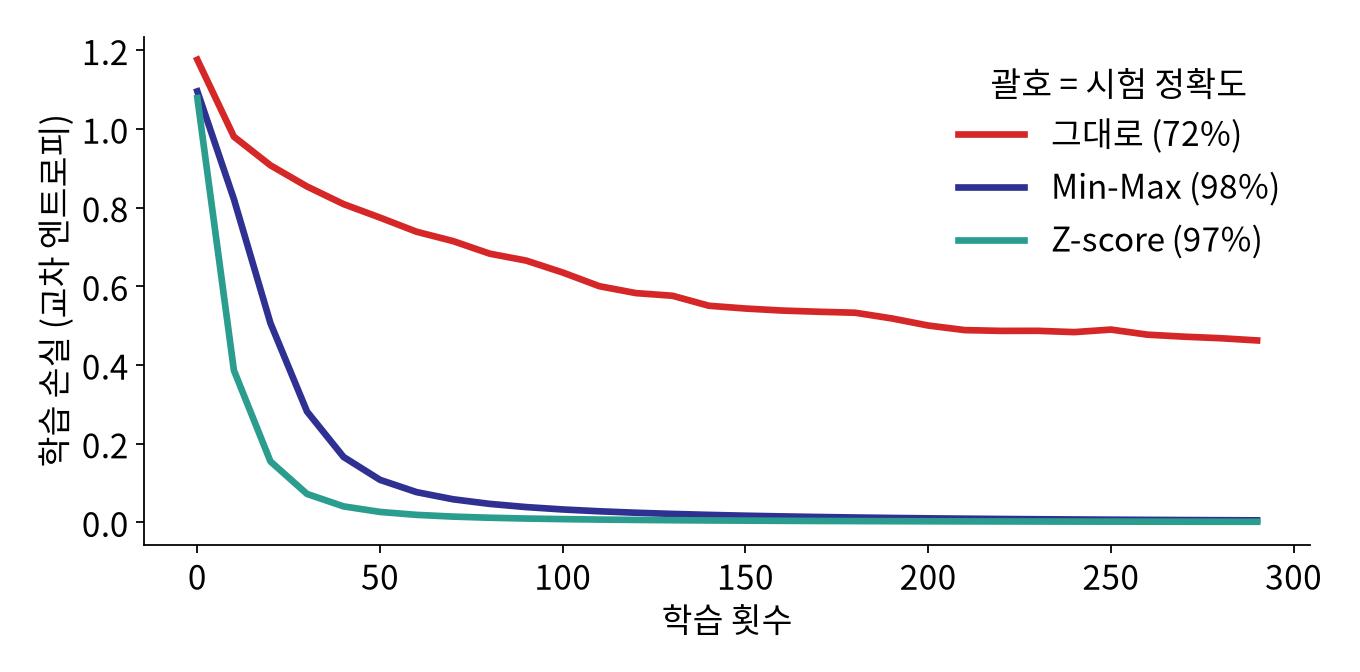
\includegraphics[width=0.64\linewidth]{fs_curve.png}\par\vskip0.3em
{\large 그대로 \kq{72\%} \quad Min-Max \kb{98\%} \quad Z-score \kb{97\%}}\\[0.3em]
{\scriptsize UCI Wine 178병, MLP 13-16-3 (tanh), 기본 초기화, Adam 0.01, 300번, 학습 70\% · 시험 30\%, 시드 10개 평균}
\vfill
\note{학습 손실 곡선입니다. 빨간 선, 그대로 넣은 경우는 300번을 돌아도 손실이 0.46에 머뭅니다. 정규화한 두 경우는 50번 만에 거의 0으로 내려갑니다. 시험 정확도는 그대로 72, Min-Max 98, Z-score 97퍼센트입니다. 여기서는 두 방법이 거의 같습니다. 중요한 건 어느 방법이냐보다, 맞추느냐 안 맞추느냐입니다.}
\end{frame}

% --- 학습 데이터로만
\begin{frame}{평균 · 표준편차는 학습 데이터로만 구한다}
\vfill
\centering
{\large
\begin{tabular}{lll}
\textbf{단계} & \textbf{할 일} & \\[0.2em]\hline\\[-0.6em]
학습 데이터 & $\mu, \sigma$ (또는 min, max) 를 \kb{구한다} & \texttt{fit}\\[0.4em]
학습 데이터 & 그 값으로 바꾼다 & \texttt{transform}\\[0.4em]
시험 · 새 데이터 & \kb{같은} $\mu, \sigma$ 로 바꾼다 (새로 구하지 않는다) & \texttt{transform}
\end{tabular}}\vskip1em
{\large 시험 데이터로 평균을 구하면 \kq{시험 문제를 미리 엿본 것} (데이터 누수)}\vskip0.8em
{\small 회귀에서 정답 $y$ 도 표준화했다면, 예측값은 마지막에 $\hat y = \hat z\,\sigma_y + \mu_y$ 로 원래 단위로 되돌린다}
\vfill
\note{중요한 규칙이 하나 있습니다. 평균과 표준편차는 학습 데이터로만 구합니다. 사이킷런으로 말하면 학습 데이터에 fit, 학습과 시험 데이터 모두에 같은 값으로 transform입니다. 시험 데이터로 평균을 다시 구하면 시험 문제를 미리 엿본 셈이 됩니다. 이걸 데이터 누수라고 합니다. 실제로 서비스할 때 새로 들어오는 데이터는 한 개씩 오니까 평균을 구할 수도 없습니다. 또, 회귀에서 정답 y까지 표준화했다면 모델이 내놓은 값은 표준화된 값이니, 마지막에 표준편차를 곱하고 평균을 더해 원래 단위로 되돌려야 합니다.}
\end{frame}

% --- 데이터마다
\begin{frame}{데이터마다: ``무엇마다'' 맞추나}
\markpage{overview}
\vfill
\centering
{\normalsize
\begin{tabular}{llll}
\textbf{데이터} & \textbf{모양} & \textbf{무엇마다} & \textbf{보통 하는 일}\\[0.2em]\hline\\[-0.6em]
표 (tabular) & (행, 열) & \kb{열(성분)마다} & Z-score\\[0.35em]
흑백 이미지 & (H, W) & 이미지 전체 & $\div 255$, 그다음 평균 · 표준편차\\[0.35em]
컬러 이미지 & (H, W, 3) & \kb{채널(R, G, B)마다} & $\div 255$, 채널별 평균 · 표준편차\\[0.35em]
언어 & 단어의 줄 & 글자 표기 & 표기 맞추기, 번호는 \kq{그대로}\\[0.35em]
시계열 & (시간,) & \kb{과거만}, 또는 창마다 & 학습 기간 Z-score, 창마다 Z-score\\[0.35em]
소리 & (샘플,) & 녹음마다 & $\div 32768$, 음량 맞추기, dB\\[0.35em]
비디오 & (T, H, W, 3) & 채널마다, \kb{영상 전체로} & 이미지와 같게, 프레임마다 따로는 X
\end{tabular}}\vskip0.8em
{\large 먼저 \kq{데이터를 열어서} 모양 · 자료형 · 최솟값 · 최댓값을 본다}
\vfill
\note{지금까지는 표 데이터였습니다. 열마다 단위가 다르니 열마다 맞췄습니다. 다른 데이터는 어떨까요? 핵심 질문은 무엇마다 맞추느냐입니다. 흑백 이미지는 모든 픽셀이 같은 단위라 이미지 전체를 한꺼번에, 컬러는 R, G, B 채널마다, 언어는 숫자 크기가 아니라 표기를 맞추고, 시계열은 과거만 보고, 소리는 녹음마다 음량을 맞추고, 비디오는 영상 전체로 맞춥니다. 하나씩 실제 데이터를 열어 보겠습니다. 어떤 데이터든 첫 단계는 같습니다. 모양, 자료형, 최솟값, 최댓값을 직접 찍어 보는 겁니다.}
\end{frame}

% --- 흑백 이미지
\begin{frame}{흑백 이미지: 픽셀 0 $\sim$ 255 를 그대로 넣으면}
\vfill
\centering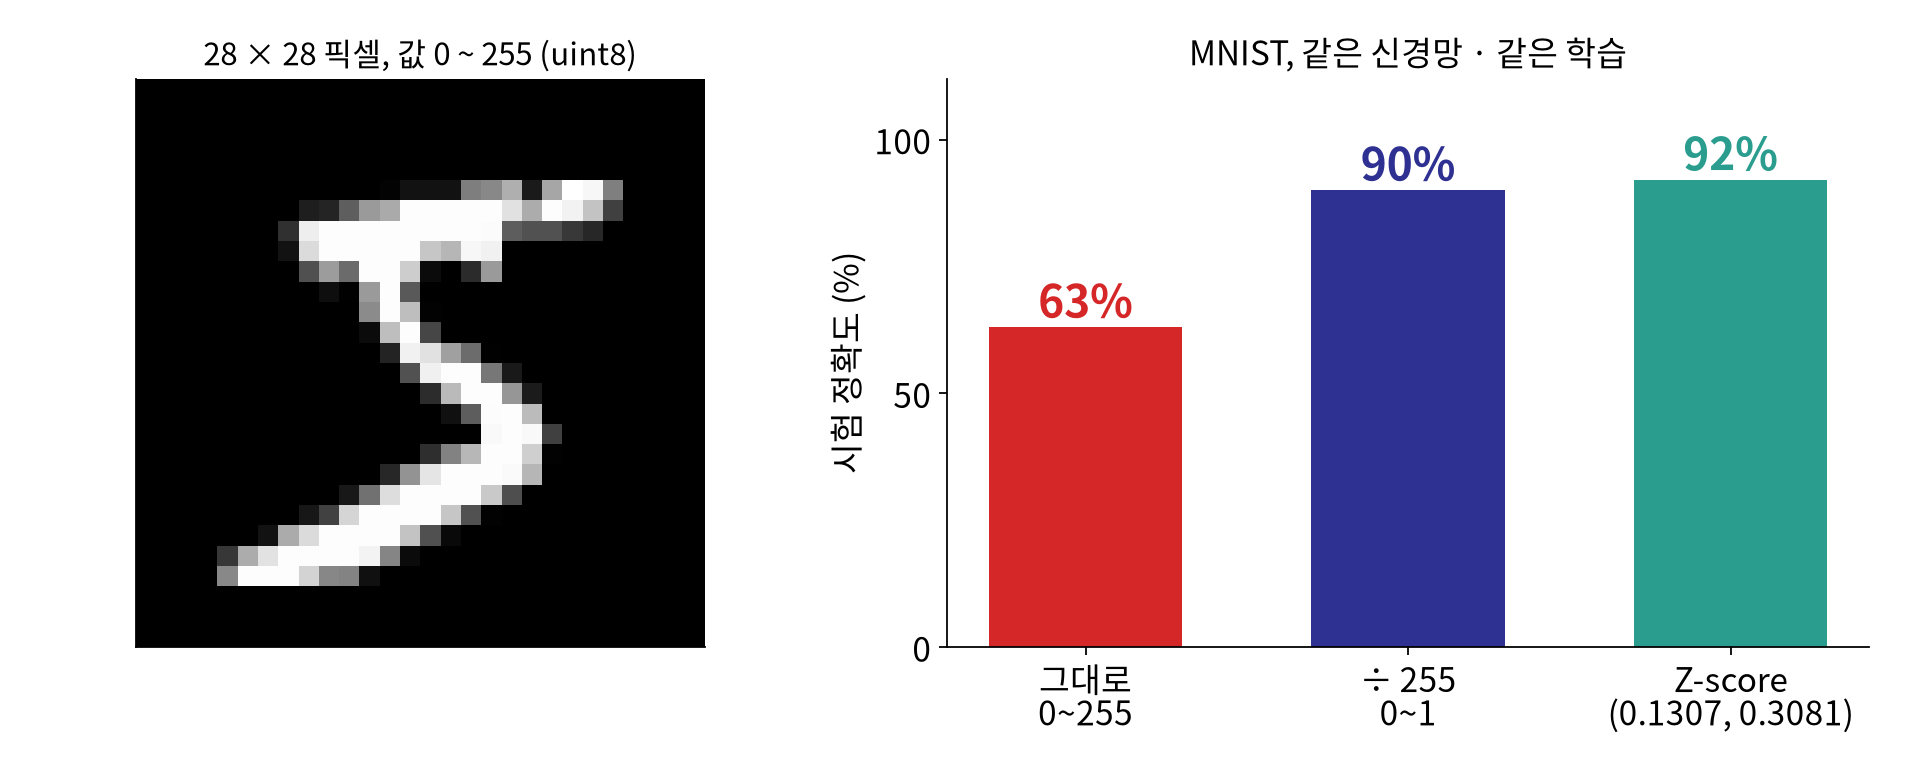
\includegraphics[width=0.82\linewidth]{fs_mnist.png}\par\vskip0.2em
{\large MNIST: $\div 255$ 만 해도 \kq{63\%} $\to$ \kb{90\%}. 그대로면 학습 전 뉴런 \kq{95\%}가 막힌다}\\[0.3em]
{\scriptsize 학습 1만 장 · 시험 1만 장, MLP 784-64-10 (tanh), SGD 0.1, 3에폭, 시드 3개 평균. 0.1307, 0.3081 = 학습 6만 장의 픽셀 평균 · 표준편차}
\vfill
\note{손글씨 숫자 MNIST입니다. 28 곱하기 28 픽셀, 값은 0에서 255 사이의 정수, 자료형은 uint8입니다. 모든 픽셀이 같은 단위라서 이미지 전체를 같은 수로 나눕니다. 그대로 넣으면 와인처럼 뉴런 95퍼센트가 막히고 정확도 63퍼센트. 255로 나누기만 해도 90퍼센트, 학습 데이터의 평균 0.1307과 표준편차 0.3081로 표준화하면 92퍼센트입니다. 한 가지 함정: uint8끼리 빼면 음수가 안 돼서, 10 빼기 20이 246이 됩니다. 계산 전에 반드시 실수형으로 바꿔야 합니다. 실습에서 직접 확인합니다.}
\end{frame}

% --- 컬러 이미지
\begin{frame}{컬러 이미지: 채널(R, G, B)마다 따로}
\vfill
\centering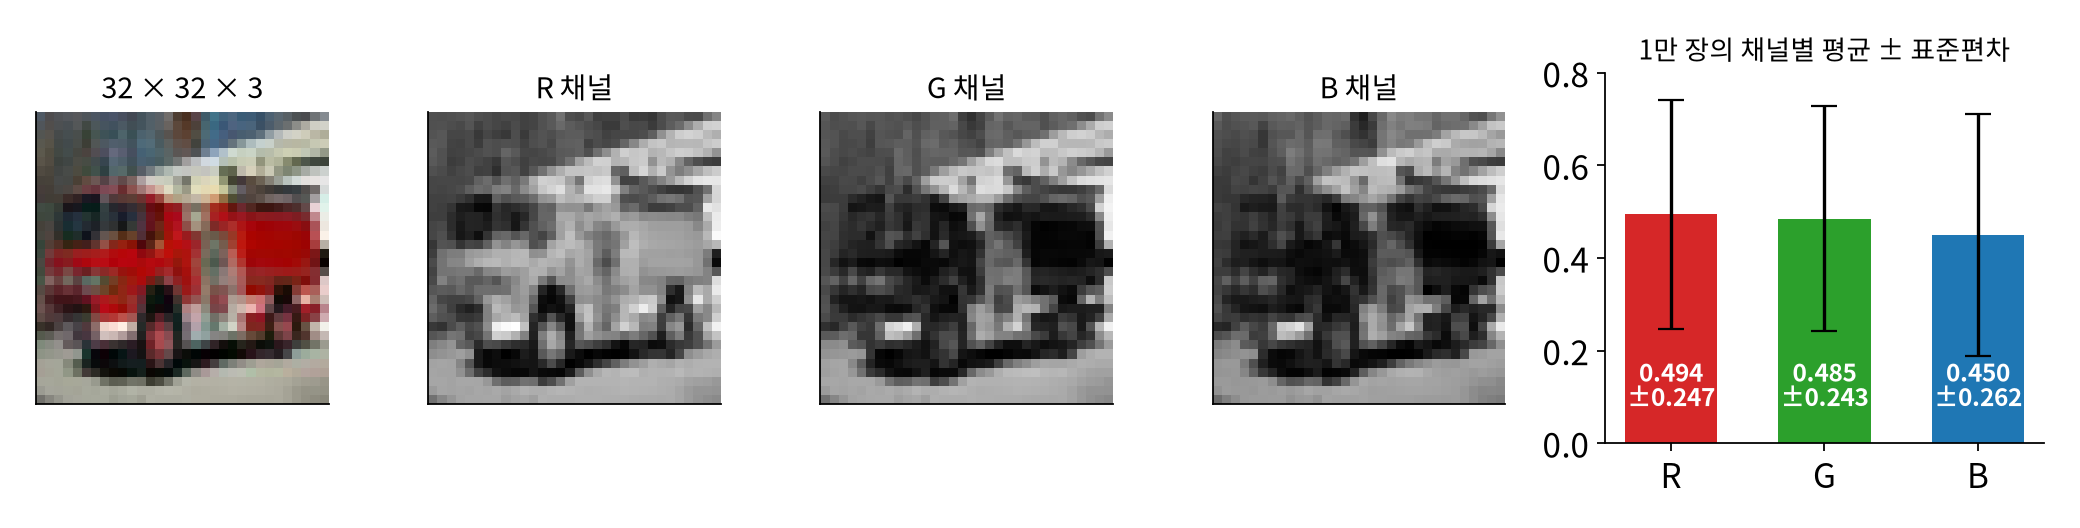
\includegraphics[width=0.94\linewidth]{fs_cifar.png}\par\vskip0.3em
{\large CIFAR-10: 평균 R \textbf{0.494}, G \textbf{0.485}, B \textbf{0.450}. 채널마다 빼고 나눈다}\\[0.4em]
{\small 사진은 (H, W, C), PyTorch 는 \kb{(C, H, W)}: 축 순서부터 확인\\[0.2em] 남이 학습시킨 모델은 그 모델의 값을 그대로 (ImageNet: 0.485, 0.456, 0.406)}
\vfill
\note{컬러 이미지는 한 픽셀에 빨강, 초록, 파랑 세 값이 있습니다. CIFAR-10 시험 이미지 1만 장으로 채널별 평균을 내면 빨강 0.494, 초록 0.485, 파랑 0.450입니다. 하늘이나 바다처럼 파란 배경도 있지만 전체로는 파랑이 조금 어둡습니다. 그래서 채널마다 따로 평균을 빼고 표준편차로 나눕니다. 결과는 숫자 세 개씩입니다. 두 가지 주의할 점. 사진 파일을 열면 높이, 너비, 채널 순서인데 파이토치는 채널을 맨 앞에 둡니다. 그리고 남이 학습시킨 모델을 가져다 쓸 때는 그 모델이 학습할 때 쓴 값, 예를 들어 ImageNet의 0.485, 0.456, 0.406을 그대로 써야 합니다.}
\end{frame}

% --- 언어
\begin{frame}{언어: 숫자 크기가 아니라 \textbf{표기}를 맞춘다}
\vfill
\centering
{\normalsize
\begin{tabular}{ll}
\kb{① 표기 맞추기} & \texttt{FREE}, \texttt{Free}, \texttt{free!} $\to$ \texttt{free}\\
& SMS 5,574통의 단어 종류 \kq{15,733} $\to$ \kb{8,713}\\[0.8em]
\kb{② 단어 번호는 크기가 아니다} & \texttt{free} $= 3373$, \texttt{call} $= 1828$: 3373 이 ``더 큰'' 단어는 아니다\\
& $\to$ 번호를 표준화하지 않는다. 임베딩 벡터로 바꾼다\\
& (\texttt{nn.Embedding} 은 처음에 평균 0, 표준편차 1 난수)\\[0.8em]
\kb{③ 단어 세기는 길이로 나누기} & 1단어 문자와 171단어 문자: 긴 글일수록 숫자가 커진다
\end{tabular}}
\vfill
\note{언어 데이터는 다릅니다. 첫째, 숫자가 아니라 글자의 표기를 맞춥니다. 대문자 FREE, 첫 글자만 대문자 Free, 느낌표 붙은 free는 모두 같은 단어입니다. 영어 문자 메시지 5,574통을 공백으로만 자르면 단어 종류가 15,733개인데, 소문자로 바꾸고 문장부호를 떼면 8,713개로 줄어듭니다. 둘째, 단어마다 번호를 붙이지만 그 번호는 크기가 아닙니다. free가 3373번이고 call이 1828번이라고 free가 더 큰 단어가 아니죠. 그래서 번호는 표준화하지 않고, 임베딩이라는 벡터로 바꿉니다. 파이토치 임베딩은 처음에 평균 0, 표준편차 1인 난수로 시작합니다. 이미 표준화된 크기에서 출발하는 셈입니다. 셋째, 단어를 세어 벡터로 만들면 긴 글일수록 숫자가 커지니, 길이로 나눠 비율로 만듭니다.}
\end{frame}

% --- 시계열
\begin{frame}{시계열: 미래는 과거의 범위를 넘는다}
\vfill
\centering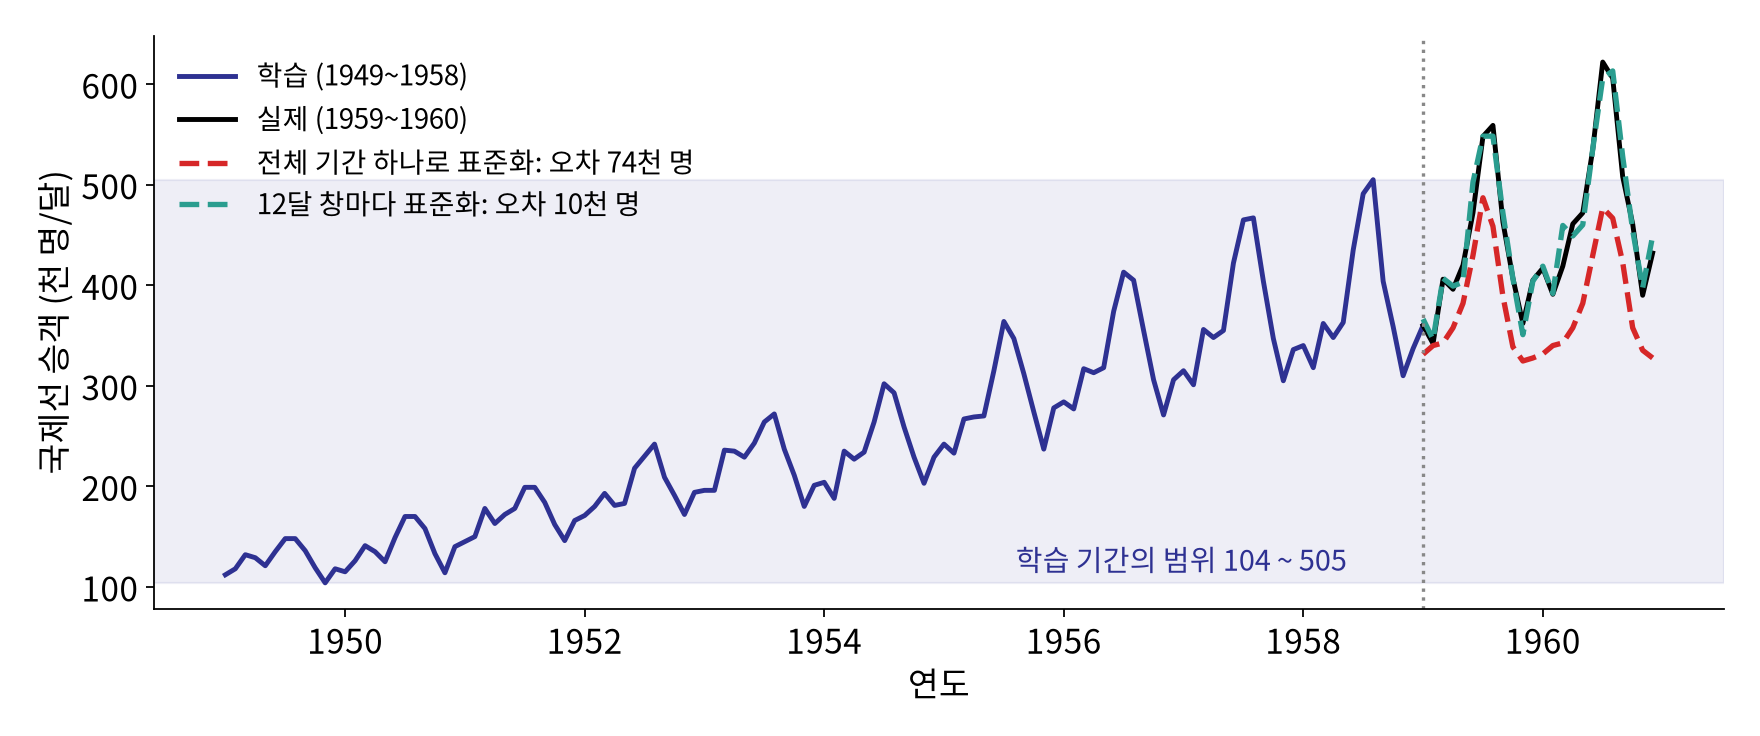
\includegraphics[width=0.8\linewidth]{fs_air.png}\par\vskip0.2em
{\large 학습 최대 505 $\to$ 시험 \kq{622} (Min-Max \kq{1.29}) \quad 창마다 표준화: 오차 \kq{74} $\to$ \kb{10}천 명}\\[0.3em]
{\scriptsize 국제선 항공 승객 1949$\sim$1960, 앞 10년 학습 · 뒤 2년 시험, 지난 12달 $\to$ 다음 달, $k$-최근접 이웃 ($k = 3$)}
\vfill
\note{시계열은 시간 순서가 있는 데이터입니다. 1949년부터 1960년까지 한 달 국제선 승객 수입니다. 앞 10년으로 학습하고 뒤 2년을 예측합니다. 규칙대로 학습 기간으로만 평균과 표준편차를 구합니다. 그런데 승객은 계속 늘어서, 학습 기간 최대가 505인데 시험 기간에는 622까지 갑니다. Min-Max로 바꾸면 1.29, 1을 넘습니다. 과거에서 가장 비슷한 패턴을 찾아오는 최근접 이웃 모델은 본 적 없는 크기를 내놓지 못해서, 빨간 점선처럼 낮게 예측합니다. 오차가 평균 74천 명. 해결책은 12달 창마다 그 창의 평균과 표준편차로 표준화하는 겁니다. 그러면 모델은 크기가 아니라 모양, 여름에 오르고 겨울에 내리는 패턴을 배웁니다. 예측한 뒤 그 창의 평균과 표준편차로 되돌리면 오차가 10천 명으로 줄어듭니다.}
\end{frame}

% --- 소리
\begin{frame}{소리: 녹음마다 음량이 다르다}
\vfill
\centering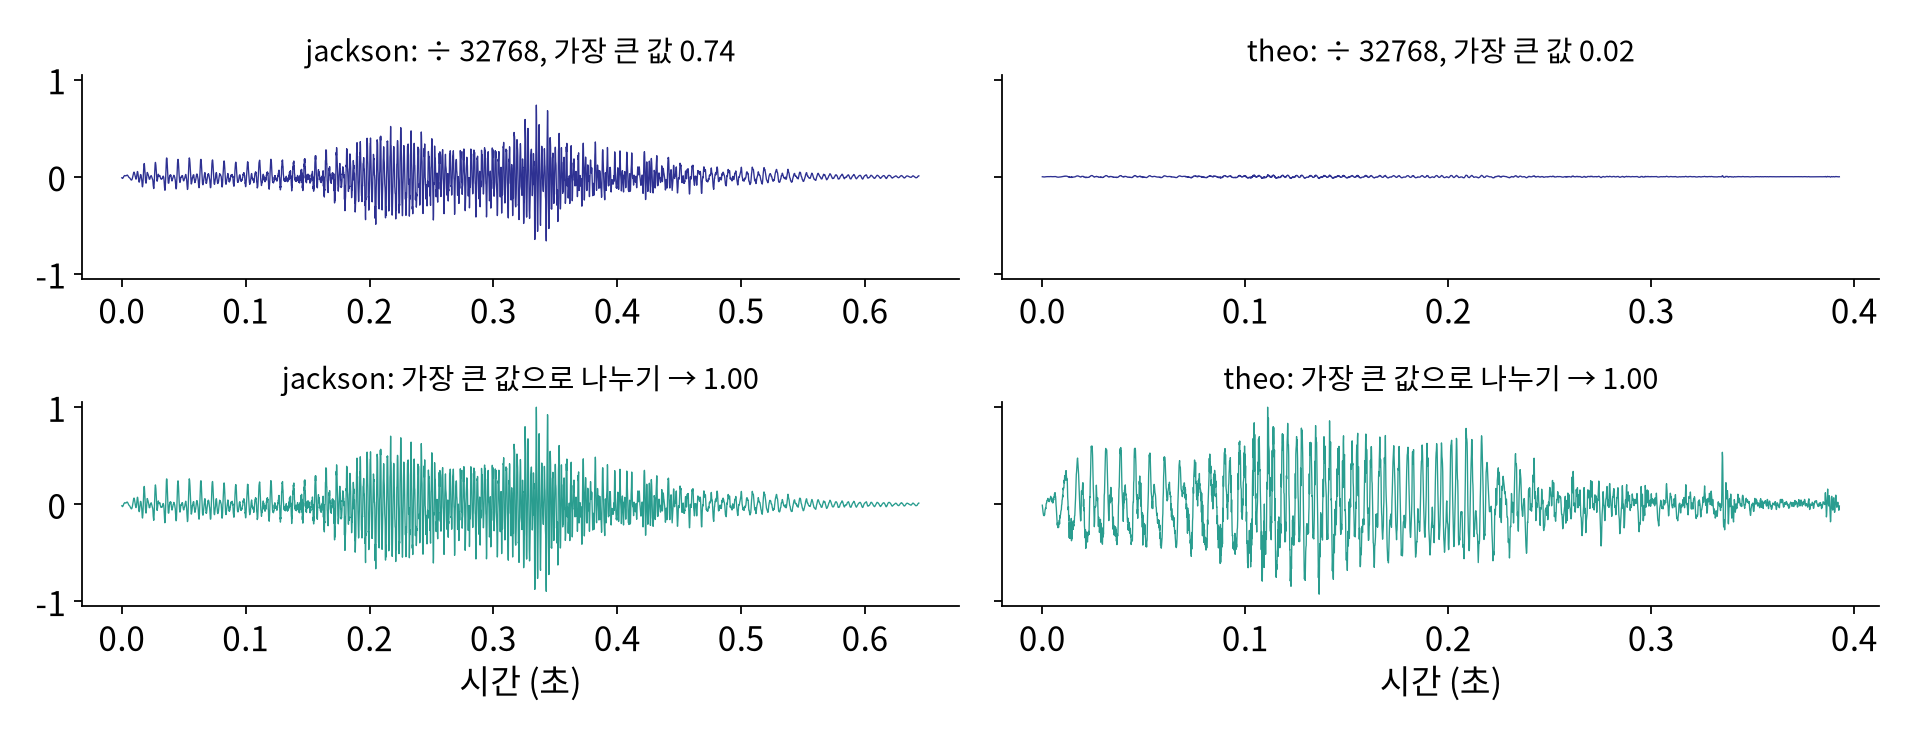
\includegraphics[width=0.84\linewidth]{fs_sound.png}\par\vskip0.2em
{\large 같은 ``zero'', 음량 \kq{37배} 차이. int16 $\div\, 32768 \to -1 \sim 1$, 그다음 \kb{녹음마다} 맞춘다}\\[0.3em]
{\scriptsize Free Spoken Digit Dataset, 8,000 Hz. 가장 큰 값으로 나누기 = 피크 정규화 (녹음마다 표준편차로 나누는 방법도 쓴다)}
\vfill
\note{소리 파일은 1초에 8,000번, 마이크가 받은 압력을 숫자로 적은 것입니다. 자료형은 16비트 정수 int16, 범위가 마이너스 32,768에서 32,767입니다. 먼저 32,768로 나눠 마이너스 1에서 1로 만듭니다. 그런데 같은 zero라는 말인데, 잭슨의 녹음은 가장 큰 값이 0.74, 테오는 0.02입니다. 37배 차이. 마이크와 거리 차이일 뿐 말의 내용은 같습니다. 그래서 녹음마다 가장 큰 값으로 나누면 둘 다 1이 되고 모양을 비교할 수 있습니다.}
\end{frame}

% --- 스펙트로그램
\begin{frame}{소리: 주파수로 바꾸면 \textbf{로그(dB)}로 본다}
\vfill
\centering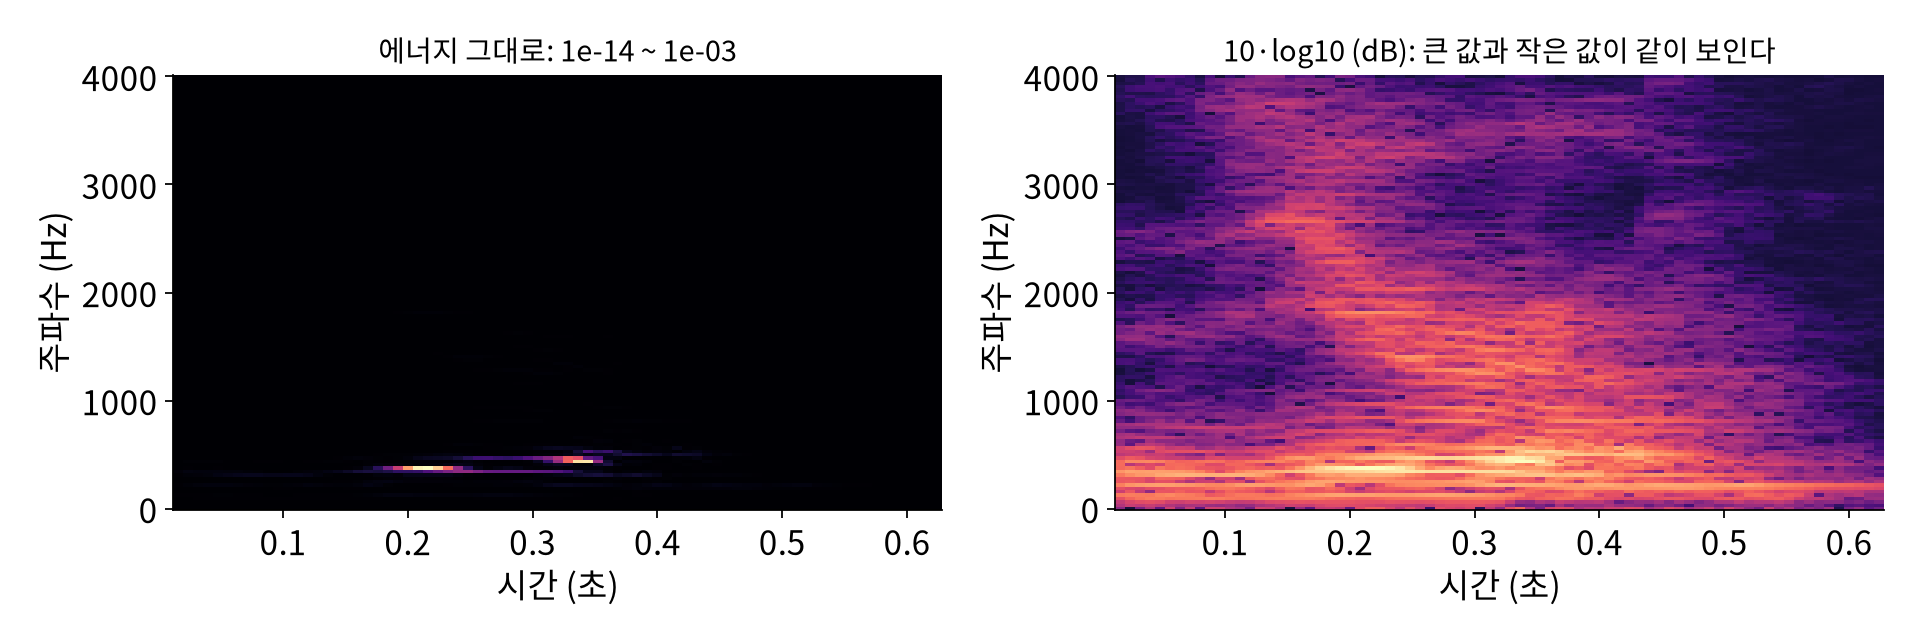
\includegraphics[width=0.84\linewidth]{fs_spec.png}\par\vskip0.3em
{\large 에너지가 $10^{-14} \sim 10^{-3}$, \kq{천억 배} 차이 $\to$ $10\log_{10}$ 로 바꿔야 작은 소리도 보인다}\\[0.3em]
{\small 음성 모델은 보통 이 dB 스펙트로그램을 다시 평균 0, 표준편차 1 로 맞춰 넣는다}
\vfill
\note{음성 인식 모델은 소리를 주파수별 에너지 그림, 스펙트로그램으로 바꿔서 넣는 경우가 많습니다. 왼쪽은 에너지를 그대로 그린 겁니다. 값이 10의 마이너스 14승에서 10의 마이너스 3승까지, 천억 배 차이가 나서 가장 센 몇 점만 보이고 나머지는 까맣습니다. 오른쪽처럼 로그를 씌워 데시벨로 바꾸면 곱하기가 더하기가 되어 작은 소리도 보입니다. 사람의 귀도 소리 크기를 로그로 느낍니다. 값이 한쪽으로 크게 치우치면, 표준화 전에 로그부터 생각합니다.}
\end{frame}

% --- 비디오
\begin{frame}{비디오: 이미지 $\times$ 시간, \textbf{영상 전체}로 맞춘다}
\vfill
\centering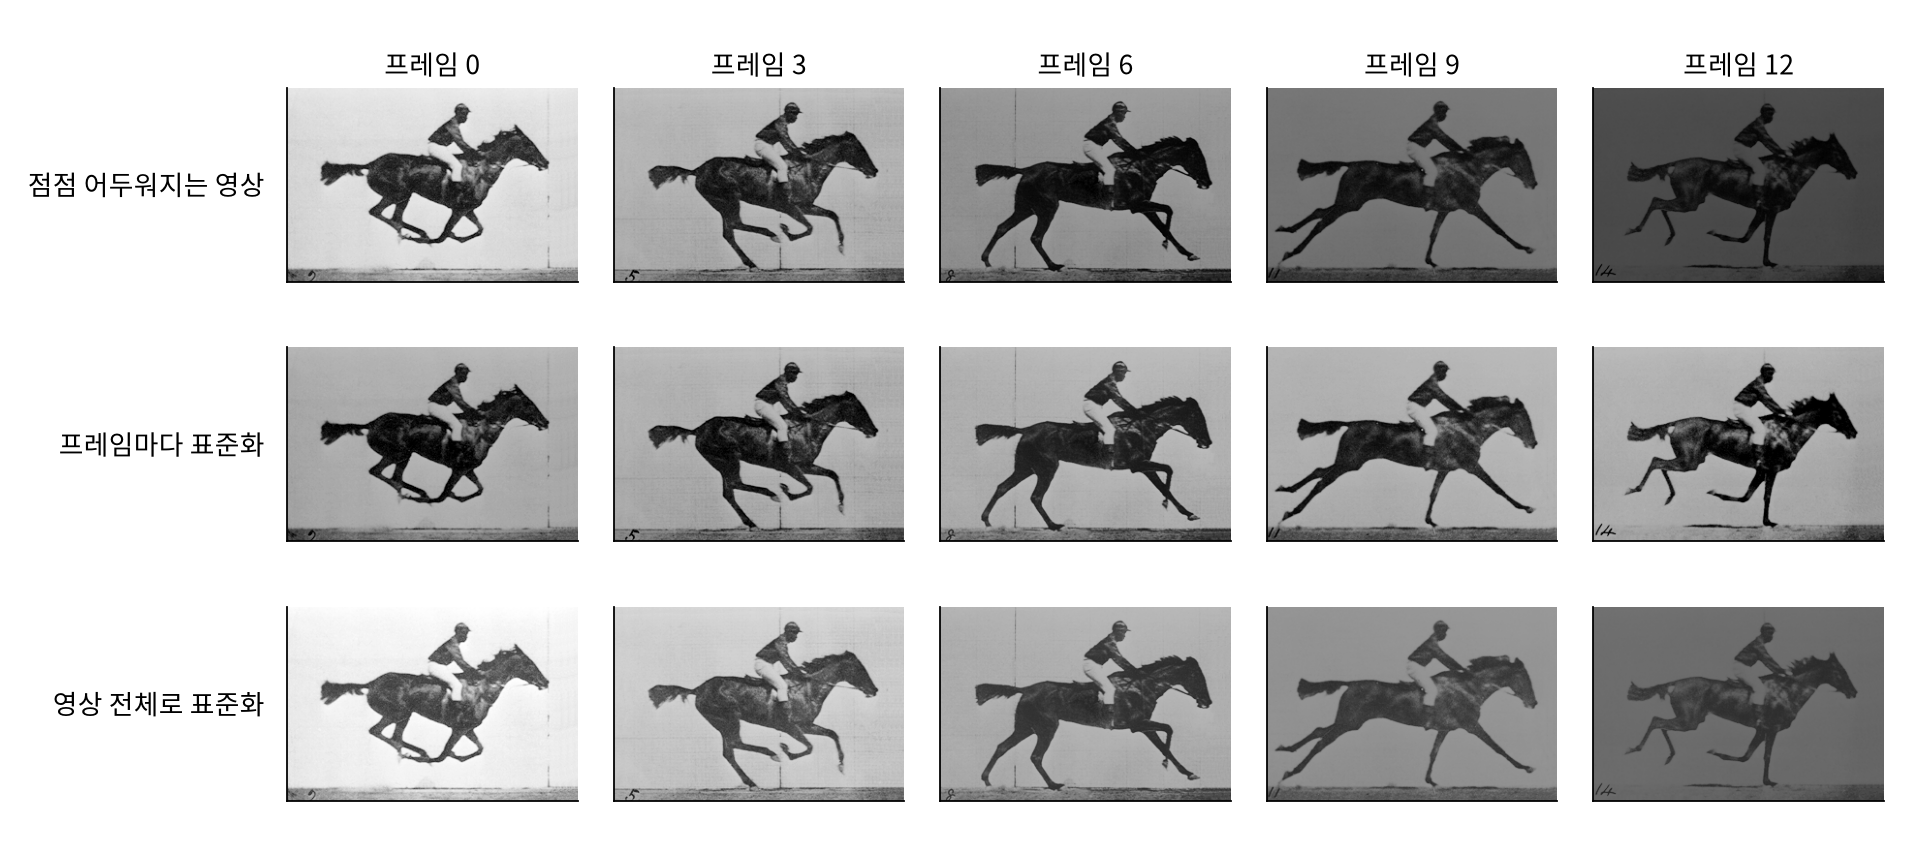
\includegraphics[width=0.76\linewidth]{fs_video.png}\par\vskip0.2em
{\large (T, H, W, C) = (15, 200, 300, 3). 프레임마다 표준화하면 \kq{어두워지는 변화가 사라진다}}\\[0.3em]
{\scriptsize Muybridge, \textit{The Horse in Motion} (1878). 실습에서는 일부러 점점 어둡게 만든 영상으로 비교}
\vfill
\note{비디오는 이미지를 시간 순서로 쌓은 것입니다. 1878년 머이브리지가 찍은 달리는 말, 15프레임, 높이 200, 너비 300, 채널 3. 처리는 이미지와 같이 255로 나누고 채널별 평균과 표준편차로 맞춥니다. 다만 그 평균을 어디서 구하느냐가 중요합니다. 첫 줄은 일부러 점점 어둡게 만든 영상입니다. 둘째 줄처럼 프레임마다 따로 표준화하면 모든 프레임이 같은 밝기가 되어 해가 지는 변화가 사라집니다. 셋째 줄처럼 영상 전체, 더 정확히는 학습 데이터 전체의 값으로 맞추면 변화가 남습니다. 밝기 변화가 중요한 문제라면 프레임마다 따로 맞추면 안 됩니다.}
\end{frame}

% --- 문제풀이
\begin{frame}{문제풀이}
\vfill
\begin{enumerate}
\item 8명의 하루 공부 시간 \texttt{[2, 4, 4, 4, 5, 5, 7, 9]}. 평균과 표준편차($n$ 으로 나눔)는? 9시간의 Z-score 는? 5시간의 Min-Max 값은?\vskip0.6em
\item 학습 데이터의 키 최솟값 150, 최댓값 190 으로 Min-Max 를 만들었다. 시험 데이터에 키 200 이 나오면 값은? 시험 데이터로 min, max 를 다시 구해야 할까?\vskip0.6em
\item \texttt{np.uint8(10) - np.uint8(20)} 은 얼마일까? 픽셀에서 평균을 빼기 전에 무엇을 해야 할까?\vskip0.6em
\item 컬러 이미지 1만 장이 \texttt{X.shape == (10000, 32, 32, 3)}. 채널별 평균을 구하려면 \texttt{X.mean(axis=?)} ? 결과는 숫자 몇 개?\vskip0.6em
\item 단어 번호(\texttt{free} = 3373)를 Z-score 로 바꿔 넣으면 왜 안 될까?
\end{enumerate}
\vfill
\note{1번 답. 합이 40이라 평균 5. 평균과의 차를 제곱하면 9, 1, 1, 1, 0, 0, 4, 16, 합 32, 8로 나누면 분산 4, 표준편차 2. 9시간은 9 빼기 5 나누기 2, Z-score 2입니다. 5시간의 Min-Max는 5 빼기 2 나누기 7, 7분의 3, 약 0.43. 2번 답. 200 빼기 150 나누기 40, 1.25입니다. 1을 넘어도 괜찮습니다. 시험 데이터로 다시 구하면 안 됩니다. 학습 때와 다른 자로 재는 셈이고 데이터 누수입니다. 3번 답. 246입니다. uint8은 0에서 255만 담을 수 있어서 음수가 되면 256을 더한 값으로 돌아갑니다. 먼저 astype float32로 바꿉니다. 4번 답. axis 0, 1, 2. 장, 높이, 너비 방향으로 평균을 내고 채널만 남기니 숫자 3개입니다. 5번 답. 번호는 이름표일 뿐 크기 정보가 없습니다. 표준화하면 3373번이 1828번보다 큰 단어인 것처럼 모델이 받아들입니다. 임베딩으로 바꿉니다.}
\end{frame}

% --- 실습
\begin{frame}[fragile]{실습: 일곱 가지 데이터를 직접 열어 보기}
\vfill
\centering\begin{tabular}{rl}
\large 1 & 표: 와인 13성분 \texttt{describe()} $\to$ Min-Max · Z-score 구현 $\to$ \kq{72\%} vs \kb{98\%}\\[0.35em]
\large 2 & 흑백 이미지: MNIST uint8 함정, $\div 255$, 평균 · 표준편차 구하기\\[0.35em]
\large 3 & 컬러 이미지: CIFAR-10 채널별 평균 · 표준편차, (H, W, C) $\to$ (C, H, W)\\[0.35em]
\large 4 & 언어: SMS 표기 맞추기 (15,733 $\to$ 8,713), 단어 세기 길이로 나누기\\[0.35em]
\large 5 & 시계열: 항공 승객, 학습 기간으로만 vs 창마다 표준화 (\kq{74} $\to$ \kb{10})\\[0.35em]
\large 6 & 소리: 숫자 말소리 6명, $\div 32768$, 음량 맞추기, dB 스펙트로그램\\[0.35em]
\large 7 & 비디오: 달리는 말 GIF, 프레임마다 vs 영상 전체
\end{tabular}\vskip0.8em
데이터는 첫 셀에서 내려받기 (MNIST · CIFAR-10 은 수십 MB) \\[0.3em]\href{https://colab.research.google.com/github/SuminHan/book-ml/blob/main/slides/v2/ml1/week01/feature_scaling/lab/feature_scaling.ipynb}{\textcolor{ksagolddk}{▶ Colab에서 실습 노트북 열기}}
\vfill
\note{실습에서는 오늘 본 일곱 가지 데이터를 직접 열어 봅니다. 순서는 매번 같습니다. 먼저 모양, 자료형, 최솟값, 최댓값을 찍어 보고, 무엇마다 맞출지 정한 뒤, 함수를 직접 만들어 바꾸고, 바꾼 뒤의 평균과 표준편차가 0과 1이 됐는지 확인합니다. 와인과 MNIST, 항공 승객에서는 정규화 전후의 결과 차이도 직접 재현합니다.}
\end{frame}

% --- 정리
\begin{frame}{정리}
\vfill
\centering\large\begin{tabular}{l}
값의 크기가 제각각이면 뉴런이 \kq{막힌다} (tanh 출력 1.00, 기울기 0)\\[0.45em]
Min-Max $\dfrac{x-\min}{\max-\min}$ \quad Z-score $\dfrac{x-\mu}{\sigma}$ \quad 통계는 \kb{학습 데이터로만}\\[0.7em]
\kb{무엇마다} 맞출지는 데이터가 정한다: 열 · 채널 · 녹음 · 창 · 영상 전체\\[0.45em]
번호(단어 id)는 크기가 아니다, 치우친 값(소리 에너지)은 로그부터\\[0.45em]
어떤 데이터든 먼저 \kq{열어서} 모양 · 자료형 · 최솟값 · 최댓값을 본다
\end{tabular}
\vfill
\note{정리합니다. 입력 값의 크기가 제각각이면 작은 난수로 시작한 뉴런이 곡선 끝에 붙어 배우지 못합니다. 성분마다 Min-Max나 Z-score로 맞추면 신호가 살아납니다. 통계는 학습 데이터로만 구합니다. 무엇마다 맞출지는 데이터가 정합니다. 표는 열마다, 컬러 이미지는 채널마다, 소리는 녹음마다, 시계열은 창마다, 비디오는 영상 전체로. 단어 번호처럼 크기가 없는 숫자는 건드리지 않고, 소리 에너지처럼 크게 치우친 값은 로그부터 씌웁니다. 무엇보다, 어떤 데이터를 받든 먼저 열어서 모양과 자료형, 최솟값과 최댓값을 직접 보세요.}
\end{frame}

% --- 이미지 출처
\begin{frame}{이미지 · 데이터 출처}
\vfill
\small
\begin{itemize}
\item 뉴런 그림: Wikimedia Commons ``Neuron.svg'' (Dhp1080, CC BY-SA 3.0), 라벨 선을 지워 사용
\item 달리는 말: Eadweard Muybridge, \textit{The Horse in Motion} (1878), 퍼블릭 도메인 (Wikimedia Commons)
\item 와인: UCI Wine (Aeberhard \& Forina, 1991) \quad 손글씨 숫자: MNIST (LeCun, Cortes, Burges)
\item 컬러 사진: CIFAR-10, A. Krizhevsky (2009) ``Learning Multiple Layers of Features from Tiny Images''
\item 문자 메시지: UCI SMS Spam Collection (Almeida \& Hidalgo, 2011)
\item 항공 승객: Box \& Jenkins, \textit{Time Series Analysis} (1976), 1949$\sim$1960 국제선 월별 승객
\item 말소리: Free Spoken Digit Dataset (Z. Jackson 외, CC BY-SA 4.0)
\end{itemize}
\vfill
\note{이 덱에 쓴 그림과 데이터의 출처입니다.}
\end{frame}
\end{document}
